\documentclass[varwidth=true, border=2pt]{standalone}

\usepackage{pgfplots}
\usepackage{tikz}

\usetikzlibrary{calc,patterns,angles,quotes}

\begin{document}
	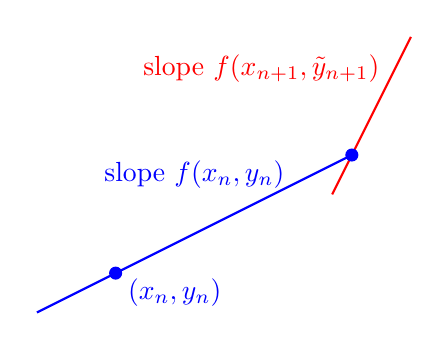
\begin{tikzpicture}
	\node (O) at (0,0) {};
	\node (B) at (3.75,1.5) {};
	\node (C) at (4,2) {};
	\node (D) at (4.75,3.5) {};

	\node [red](RISe) at (2.85,3.1) {slope $f(x_{n+1},\tilde y_{n+1})$};
	\node [blue](O1) at (1.75,0.25){($x_n,y_n)$};
	\node [blue](C1) at (2,1.75){slope $f(x_n,y_n)$};

	\draw [thick,blue] (O.center) to (C.center);
	\draw [thick,red] (B.center) to (D.center);

	\draw[blue,fill=blue] (1,0.5) circle (.5ex);
	\draw[blue,fill=blue] (4,2) circle (.5ex);
	\end{tikzpicture}
\end{document}